\documentclass[subeqn]{article}

\title{The Twin Instrument\footnote{We are grateful to Paul Devereux, 
James Fenske, Cheti Nicoletti, Atheen Venkataramani and Marcos Vera-Hernandez, 
along with seminar audiences and discussants at CMPO Bristol, ESPE, NEUDC, CSAE, 
The University of Essex, The University of Oxford and the Barcelona GSE summer 
forum for helpful comments.  We also are indebted to Emilia Del Bono, Climent 
Quintana-Domeque, Pedro R\'odenas, Libertad Gonz\'alez, Anna Aevarsdottir,
Martin Foureaux Koppensteiner and Ryan Palmer who have very kindly shared data 
and source code from their work.}}
\author{Sonia Bhalotra\thanks{The University of Essex.
Contact: srbhal@essex.ac.uk} 
\and Damian Clarke\thanks{The University of Oxford. 
Contact: damian.clarke@economics.ox.ac.uk}}
\date{\today}


%*******************************************************************************
\usepackage{amsmath}
\usepackage{amssymb}
\usepackage{appendix}
\usepackage{blindtext}
\usepackage{bm}
\usepackage{booktabs}
\usepackage{breqn}
\usepackage{caption}
\usepackage{color} \pagecolor{white}
\usepackage{dcolumn}
\usepackage{epsfig}
\usepackage{epstopdf}
\usepackage[capposition=top]{floatrow}
\usepackage{lastpage}
\usepackage{longtable}
\usepackage{lscape}
\usepackage{multirow}
\usepackage{natbib} \bibliographystyle{abbrvnat}\bibpunct{(}{)}{;}{a}{,}{,}
\usepackage{pdfpages}
\usepackage{rotating}
\usepackage{setspace}
\usepackage{subcaption}
\usepackage{url}
\usepackage{wrapfig}


%*******************************************************************************
\setlength\topmargin{-0.375in}
\setlength\textheight{8.8in}
\setlength\textwidth{5.8in}
\setlength\oddsidemargin{0.4in}
\setlength\evensidemargin{-0.5in}
\setlength\parindent{0.25in}
\setlength\parskip{0.25in}

\newcommand{\twinfolder}{"/home/damiancclarke/investigacion/Activa/Twins"}

%*******************************************************************************
\begin{document}
\begin{spacing}{1.4}

\maketitle
\begin{abstract}
 The incidence of twins has been used to identify the impact of changes in 
 fertility on measures of investment in children born prior to the twins, and
 the emerging consensus in this literature is that there is no evidence of a
 quantity-quality trade-off. We argue that the standard approach is flawed.
 Even if twin conception is random, bringing twins to term is a function of
 maternal health which is difficult to fully observe and which tends to be
 correlated with child quality, rendering the instrument invalid. The neglect
 of this fact in the existing literature will tend to lead to
 under-estimation of the quality-quantity (Q-Q) trade-off and so could
 contribute to explaining the negative results in the literature. Our contention
 that women who produce twin births are positively selected is demonstrated using
 data from richer and poorer countries. Using a large sample of microdata from
 developing countries which include indicators of maternal characteristics
 including health, we show that a significant trade-off emerges upon correcting
 for these biases. We show that this result is likely to be only a \emph{lower}
 bound of the true Q-Q trade-off and discuss how to estimate the size of these
 bounds.
 \\
\end{abstract}
\hspace{4mm}\textbf{\small JEL codes}: J12,J13,C13,D13,I12. \\

\newpage
%*******************************************************************************
\section{Introduction}                             \label{TWINscn:intro}
\section{The Twin Literature}                      \label{TWINscn:literature}
\section{Data and Estimation Samples}              \label{TWINscn:data}
\subsection{Data}                                  \label{TWINsscn:data}
\subsection{Estimation Samples}                    \label{TWINsscn:samples}
\subsection{Descriptive Statistics}                \label{TWINsscn:descriptives}
\section{Methodology}                              \label{TWINscn:method}
\subsection{Quantity-Quality with Twins}           \label{TWINsscn:methodQQ}
\subsection{Bounding the Q-Q Trade-off}            \label{TWINsscn:methodBounds}
\section{Results}                                  \label{TWINscn:results}
\subsection{Twinning}                              \label{TWINsscn:twinning}
Table \ref{TWINtab:TwinDHS}, \ref{TWINtab:TwinNHIS}.
Appendix tables: \ref{TWINtab:TwinNVSS}
Add as appendix table balance of characteristics.

\subsection{Selection into twinning: mechanisms}   \label{TWINsscn:selection}
In a wide variety of contexts, healthier women are more likely to give birth to
twins.  There are a number of competing hypotheses which may explain why this is
the case.  Firstly, it may simply be the case that healthier mothers are more 
likely to conceive twins.  This may reflect some underlying biological process, 
such as that mediated by follicle stimulating hormone as discussed in 
\citet{Hall2003}.  Secondly, conditional on conceiving twins, healthier mothers 
may be more likely to take both fetuses to term.  Finally, it may be the case 
that (conditional on conceiving twins and taking them to term), healthier mothers 
may be more likely to survive the birth, and hence appear in surveys or vital 
statistics data.  In broad terms we will refer to these as the conception 
mechanism, the gestation mechanism and the birth survival mechanism.

When considering instrumental estimates, any of these processes is sufficient to
invalidate causal inference insofar as observing twins now depends upon hard to
measure maternal behaviours and characteristics..  Nonetheless, we may be 
interested in determing which of these are the relevant channels to explain the
results from the previous section.  Particularly, the mechanism may be relevant
when considering the use of the instrument.  For example, if twins are less 
likely \emph{only} due to selective maternal death, then as mothers are more 
likely to survive childbirth (ie moving from high maternal mortality countries 
to low maternal mortality countries), threats to instrumental validity become 
less relevant.

We test these mechanisms below.  While credible data on twin conceptions is hard 
to come by, we are able to test each of the other two mechanisms.  Firstly, when
considering the gestation mechanism, we are able to test whether less healthy
mothers are more likely to miscarry twins.  While data on miscarriages as well
as the type of miscarriage (single or multiple fetuses), are somewhat hard to 
come by, in one DHS survey (Nepal) this is recorded.  We thus run a series of 
regressions where miscarriage is the dependent variable, and the independent
variables are a measures of poor maternal health, whether the pregnancy is 
single or multiple, and interactions between pregnancy type and poor maternal 
health.  We would expect that both poor maternal health and a non-singleton
pregnancy increase the likelihood of miscarriage, however we are interested in
determing if more unhealthy mothers are \emph{more} likely to miscarry twins
than healthy mothers carrying twins.  Thus, we are interested in testing if the
coefficients on the interaction terms are significantly larger than zero.

These regression results are reported in table \ref{TWINtab:Miscarry}.  As 
expected, columns (1) and (2) suggest that more unhealthy and less educated
women are more likely to report ever miscarrying.\footnote{These results hold 
conditional and unconditional on total fertility.}  Maternal health stocks 
are proxied by height and BMI, where (negative) outcomes for these variables
such as underweight are based on ICD definitions.  Turning to the interaction
terms, although standard errors are reasonably large due to the low frequency
of twinning, women who are unhealthy (as proxied by a very low BMI), and with
no education are significantly more likely to miscarry with twins.  Using a
richer set of variables from administrative data in the USA and Spain, similar 
regressions are run.  The results in appendix tables \ref{TWINtab:USAMiscarry}
and \ref{TWINtab:SpainMiscarry} suggest that, depending on the context, less
educated women and women who report consuming alcohol during pregnancy are
more likely to miscarry twins than mothers with higher education and who do
not consume alcohol.


\subsection{The twin instrument and the Q-Q trade-off} \label{TWINsscn:QQtwins}
\subsection{Bounding the Q-Q trade-off}            \label{TWINsscn:resultBounds}



\section{Conclusion}                               \label{TWINscn:conclusion}

\newpage
\section*{Figures}
\begin{figure}[htpb!]
\centering
\begin{subfigure}{.5\textwidth}
  \centering
  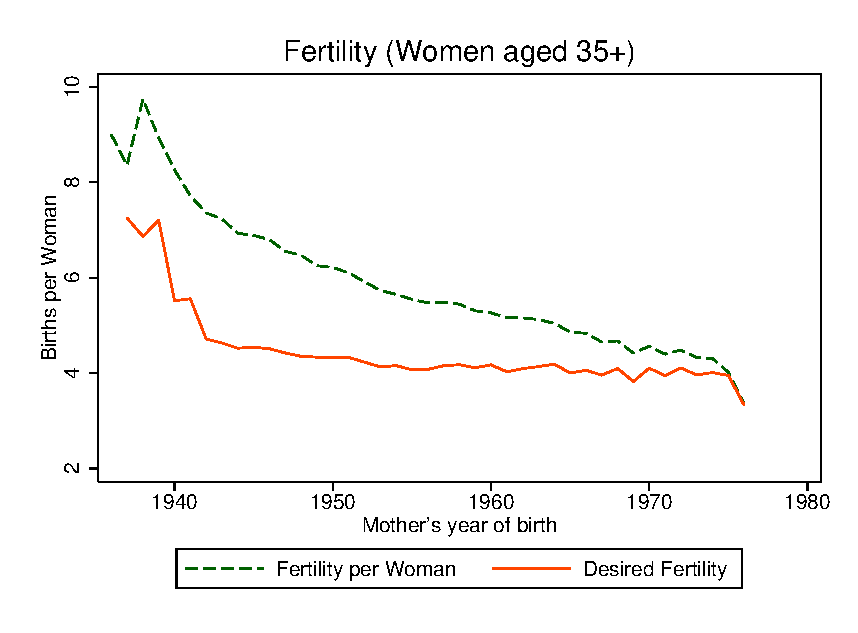
\includegraphics[scale=0.53]{\twinfolder/Figures/ferttrend_35_all.eps}
  \caption{Trends in Fertility}
  \label{TWINfig:fertrend}
\end{subfigure}%
\begin{subfigure}{.5\textwidth}
  \centering
  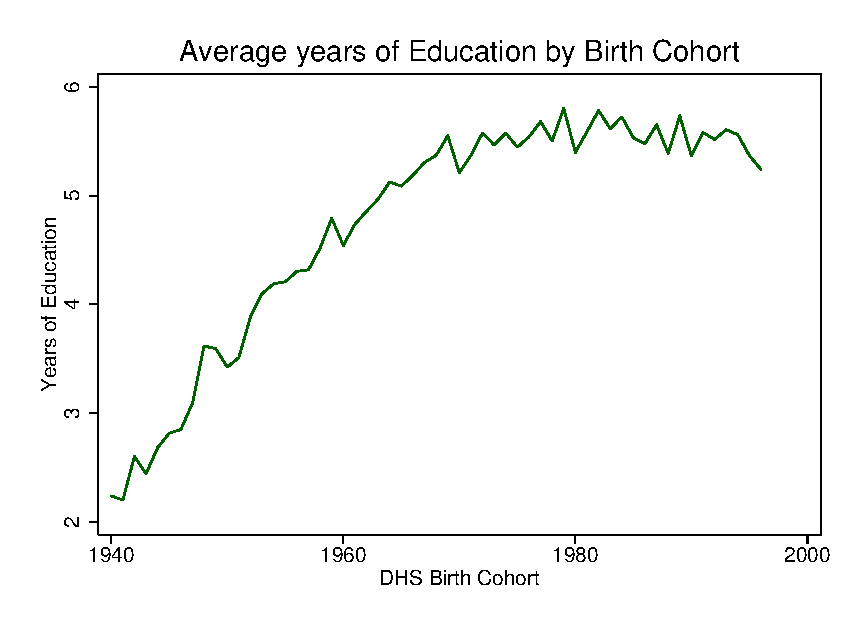
\includegraphics[scale=0.52]{\twinfolder/Figures/eductrend_all.eps}
  \caption{Trend in Education}
  \label{TWINfig:eductrend}
\end{subfigure}
\caption{Education and Fertility}
\label{TWINfig:trends}
\floatfoot{Note to figure \ref{TWINfig:trends}: Cohorts are made up of all individuals 
from the DHS who are over 35 years (for fertility), and over 15 years (for education).  
In each case the sample is restricted to those who have approximately completed fertility 
and education respectively.}
\end{figure}
\vspace{1cm}

\begin{figure}[htpb!]
\begin{center}
\caption{Proportion of Twins of All Births (USA)}
\label{TWINfig:bord}
\includegraphics[scale=0.92]{\twinfolder/Figures/USTwinFLE.eps} 
\end{center}
\end{figure}

\begin{figure}[htpb!]
\begin{center}
\caption{Twin Births and Total Fertility}
\label{TWINfig:births}
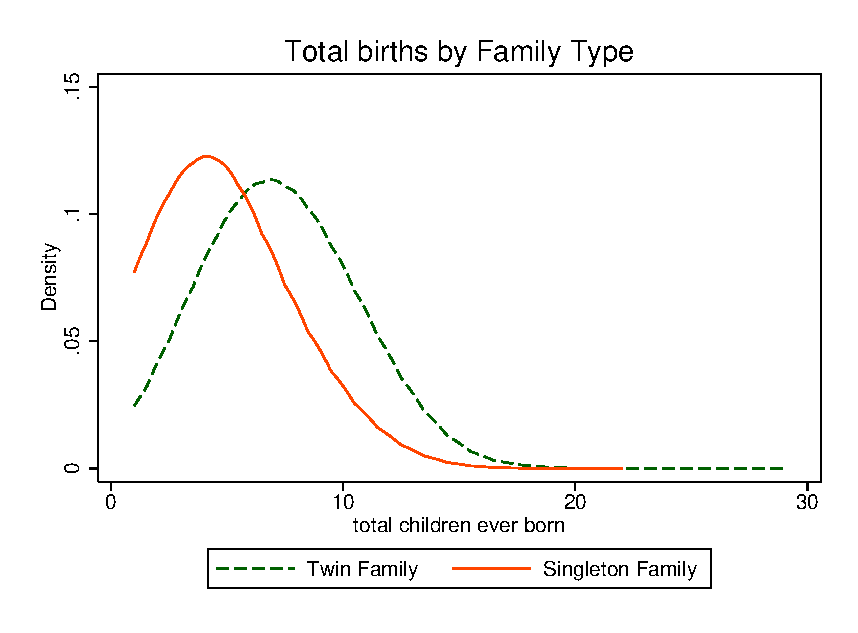
\includegraphics[scale=0.92]{\twinfolder/Figures/famsize.eps} 
\end{center}
\end{figure}

\begin{figure}[htpb!]
\begin{center}
\caption{Proportion of Twins by Birth Order}
\label{TWINfig:bord}
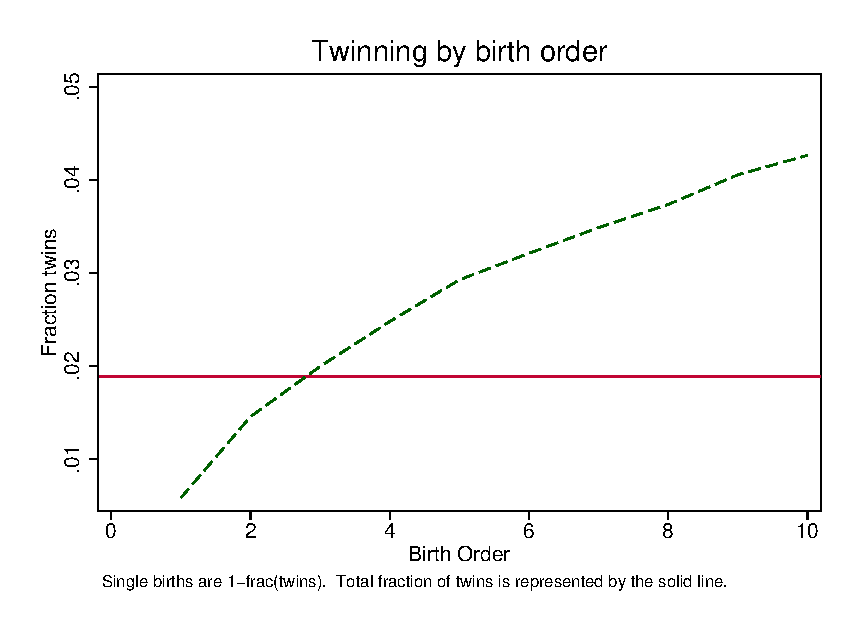
\includegraphics[scale=0.92]{\twinfolder/Figures/twinbybord.eps} 
\end{center}
\end{figure}

\begin{figure}[htpb!]
\begin{center}
\caption{Intra- and Inter-country trends: height and twinning}
\label{TWINfig:arrows}
\includegraphics[scale=0.86]{\twinfolder/Figures/height_country.eps} 
\end{center}
\end{figure}

%\begin{figure}[htpb!]
%\begin{center}
%\caption{Distribution of Ideal Family Size}
%\label{TWINfig:ideal}
%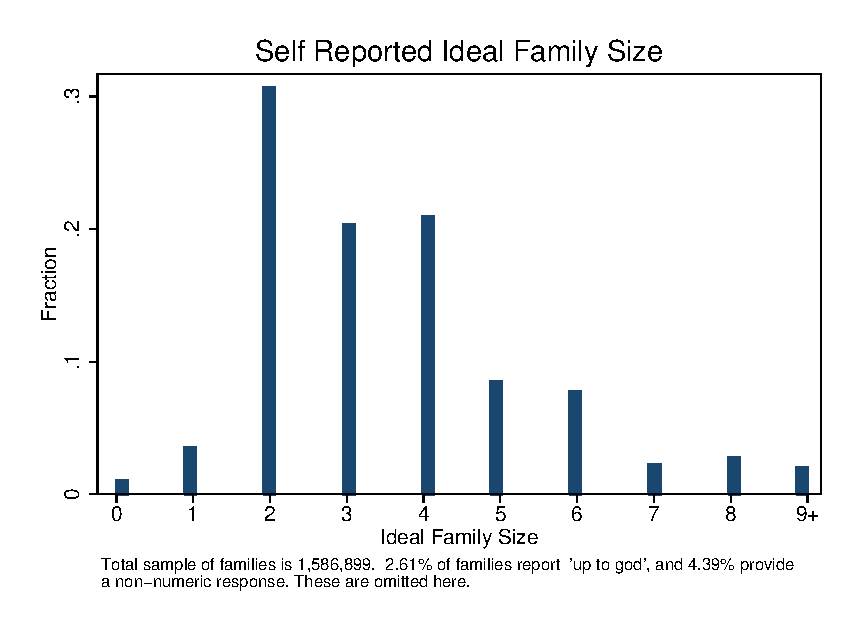
\includegraphics[scale=0.92]{\twinfolder/Figures/idealfamsize.eps} 
%\end{center}
%\end{figure}

%\begin{figure}[htpb!]
%\begin{center}
%\caption{Ideal and Actual Fertility}
%\label{TWINfig:idealactual}
%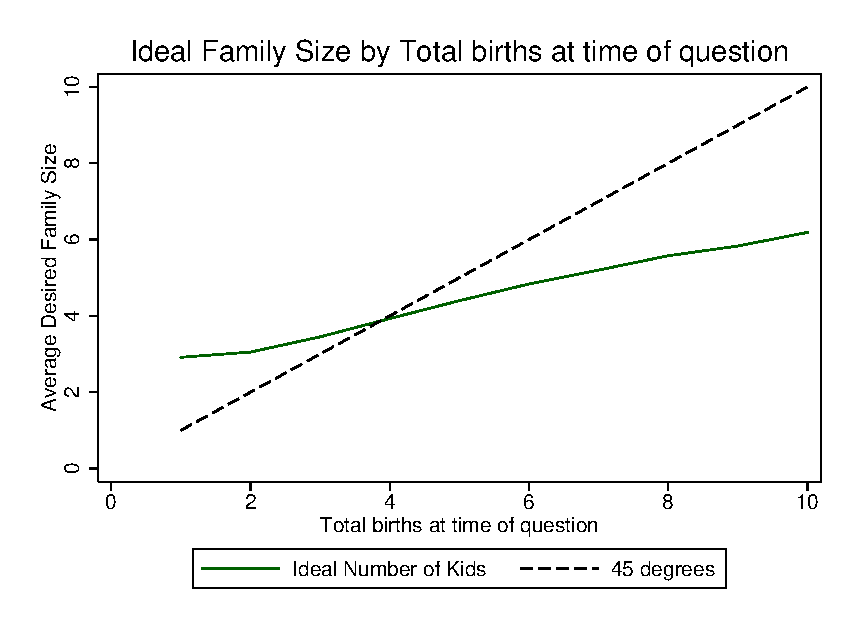
\includegraphics[scale=0.92]{\twinfolder/Figures/idealfam_fert.eps} 
%\end{center}
%\end{figure}

\begin{figure}[htpb!]
\begin{center}
\caption{Relaxing Strict Exogeneity (two plus)}
\label{TWINfig:ltz2}
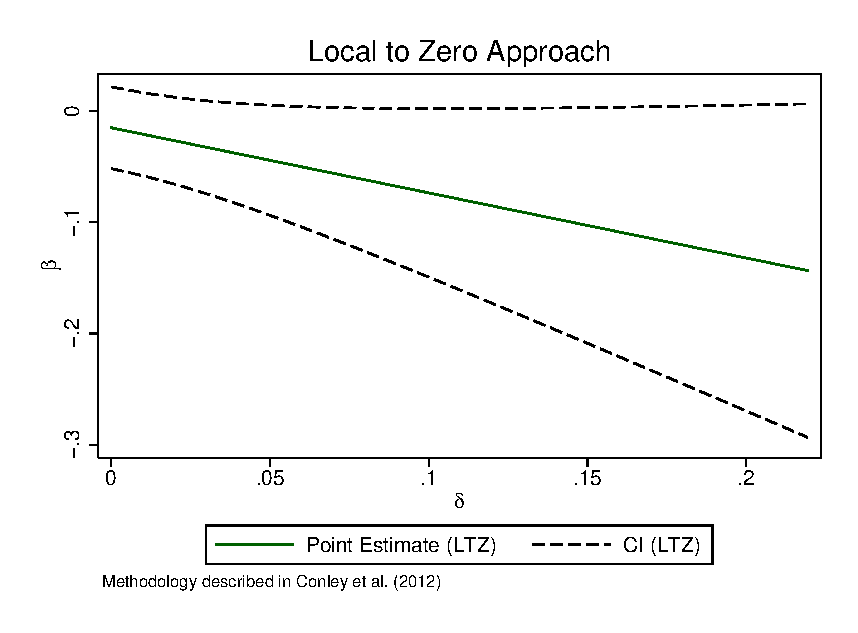
\includegraphics[scale=0.88]{\twinfolder/Figures/LTZ_two.eps}
\vspace{-8mm}
\floatfoot{Note to figure \ref{TWINfig:ltz2}: See note to Figure \ref{TWINfig:ltz3}}
\end{center}
\end{figure}

\begin{figure}[htpb!]
\begin{center}
\caption{Relaxing Strict Exogeneity (three plus)}
\label{TWINfig:ltz3}
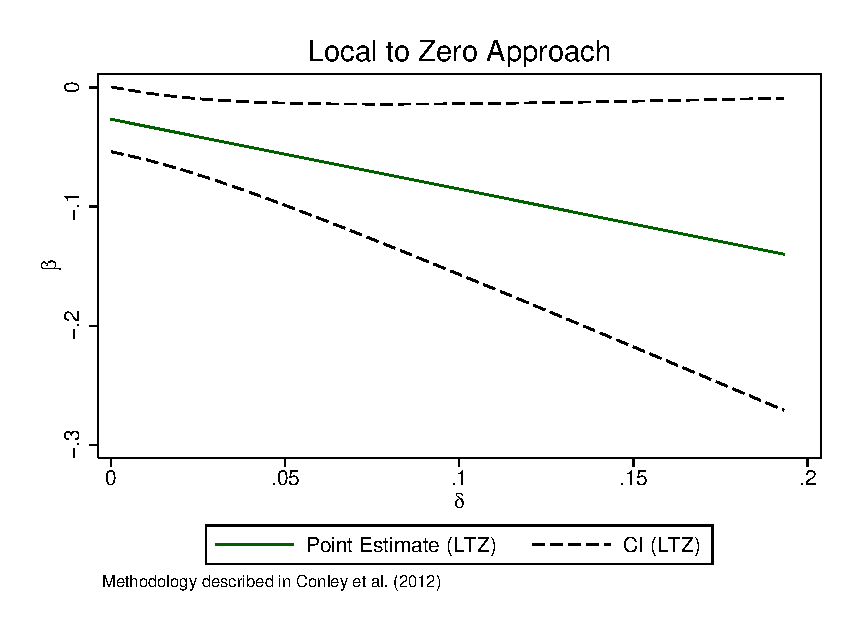
\includegraphics[scale=0.88]{\twinfolder/Figures/LTZ_three.eps} 
\floatfoot{Note to figure \ref{TWINfig:ltz3}: Confidence intervals and point estimates 
are calculated according to \citet{Conleyetal2012}.  Estimates reflect a range of priors 
regarding the validity of the exclusion restriction required to consistently estimate 
$\hat\beta_{fert}$ using twinning in a 2SLS framework.  The local to zero (LTZ) 
approach applied here assumes that $\gamma$, the sign on the instrument when included
in the first stage, is distributed $\gamma\sim U(0,\delta)$.  Further discussion 
is provided in the body of the text and table \ref{TWINtab:Conley}.}
\end{center}
\end{figure}




\clearpage
\section*{Tables}
\begin{table}[htpb!]\caption{Summary Statistics} 
\label{TWINtab:sumstats}\begin{center}\scalebox{0.99}{\begin{tabular}{lccccc}
\toprule \toprule 
&\multicolumn{2}{c}{Low Income}&\multicolumn{2}{c}{Middle Income}\\ 
\cmidrule(r){2-3} \cmidrule(r){4-5}
& Single & Twins & Single & Twins & All \\ \midrule 
\textsc{Fertility} & & & & & \\ 
Fertility&3.749&6.223&3.412&5.584&3.689\\
&(2.392)&(2.622)&(2.308)&(2.687)&(2.406)\\
Desired Family Size&4.193&5.328&3.380&4.190&3.921\\
&(2.530)&(2.885)&(2.130)&(2.555)&(2.440)\\
Fraction Twin & \multicolumn{2}{c}{  0.0200}& \multicolumn{2}{c}{  0.0179 } &  0.0191\\
& \multicolumn{2}{c}{(0.1402)}& \multicolumn{2}{c}{(0.1326)} & (0.1370)\\
Birth Order Twin & \multicolumn{2}{c}{   4.664}& \multicolumn{2}{c}{   4.016 }&   4.410\\
& \multicolumn{2}{c}{(2.465)}& \multicolumn{2}{c}{(2.374)}& (2.450)\\
\textsc{Mother's Characteristics}&&&&&\\ Age
&31.22&34.52&32.32&35.61&31.72\\
&(8.238)&(7.381)&(8.356)&(7.428)&(8.293)\\
Education&3.859&3.222&6.690&5.906&4.885\\
&(4.327)&(3.991)&(4.795)&(5.023)&(4.706)\\
Height&155.5&157.6&155.6&157.2&155.6\\
&(7.093)&(7.065)&(6.966)&(6.945)&(7.053)\\
BMI&21.90&22.50&25.90&26.63&23.39\\
&(4.027)&(4.175)&(5.118)&(5.512)&(4.867)\\
Pr(BMI)$<$18.5&0.175&0.125&0.0346&0.0276&0.122\\
&(0.380)&(0.331)&(0.183)&(0.164)&(0.327)\\
Actual Births$>$Desired&0.310&0.526&0.324&0.575&0.321\\
&(0.463)&(0.499)&(0.468)&(0.494)&(0.467)\\
\textsc{Children's Outcomes}&&&&&\\ Education (Years)
&3.660&3.204&5.445&5.043&4.446\\
&(3.576)&(3.293)&(3.867)&(3.760)&(3.810)\\
Education (Z-Score)&-0.00843&-0.0156&0.0119&-0.0428&0.000144\\
&(1.001)&(0.963)&(0.998)&(0.987)&(1.000)\\
No Education (Percent)&0.207&0.222&0.0649&0.0786&0.144\\
&(0.405)&(0.416)&(0.246)&(0.269)&(0.351)\\
Infant Mortality&0.0158&0.0917&0.00946&0.0497&0.0141\\
&(0.125)&(0.289)&(0.0968)&(0.217)&(0.118)\\
Child Mortality&0.0239&0.108&0.0122&0.0535&0.0199\\
&(0.153)&(0.310)&(0.110)&(0.225)&(0.140)\\
\midrule
Number of Countries & 39&39  & 28&28  & 67 \\
Number of Children &2,231,844 &45,654 &1,614,358 &29,430 & 3,921,286 \\
Number of Mothers &875,587 &12,908 &653,969 &8,605 & 1,586,899 \\
\midrule
\multicolumn{6}{p{13.2cm}}{\begin{footnotesize}\textsc{Notes:}  Group means are presented with standard deviation below in parenthesis.  Education is reported as total years attained, and Z-score presents educational attainment relative to country and cohort (mean 0, std deviation 1).  Infant mortality refers to the proportion of children who die before 1 year of age,  while child mortality refers to the proportion who die before 5 years.  Maternal height is reported in cm, and BMI is weight in kg over height in metres squared.  Summary statistics are for the full sample of 1,586,899
 mothers responding to any publicly available DHS survey.  For a full list of country and years of survey, see appendix table \ref{TWINtab:countries}.\end{footnotesize}} \\ \bottomrule \end{tabular}}\end{center}\end{table}


\begin{landscape}\begin{table}[htpb!]\caption{Fertility and the Twin Instrument: Literature} 
\label{TWINtab:Lit}\begin{center}\begin{tabular}{p{4cm}p{5cm}p{5cm}p{2cm}p{1.22cm}p{1.22cm}}
\toprule \toprule 
&&&&\multicolumn{2}{c}{Estimates}\\ \cmidrule(r){5-6}
Author & Data, Period & Controls Included & Sample & \ \ OLS & \ \ IV \\ \midrule 
(1) \citet{Blacketal2005} & 
Norway matched administrative files of
individuals aged 16-74 during 1986-2000,
(children $>$ 25 years). Outcome is 
completed years of education. & 
Age, parents' age, parents' education, 
sex. &  \begin{tabular}[t]{@{}l@{}} Two Plus \\ \\ Three Plus \\ \\ Four Plus \end{tabular}
& -0.060 (0.003) -0.076 (0.004) -0.059 (0.006)
& -0.038 (0.047) -0.016 (0.044) -0.024 (0.059) \\
&&&&& \\
(2) \citet{Caceres2006} & 
USA 1980 Census Five-Percent Public Use Micro Sample.
Children aged 6-16 years. Outcome (reported here) 
is an indicator of whether the child is behind his
or her cohort. & Age, state of residence, mother's
education, race, mother's age, sex. &
\begin{tabular}[t]{@{}l@{}} Two Plus \\ \\ Three Plus \end{tabular}
& 0.011 (0.000) 0.017 (0.001)
& 0.002 (0.003) 0.010 (0.006) \\
&&&&& \\
(3) \citet{Angristetal2010} & 
Israel 20\% public-use microdata samples
from 1995 and 1983 censuses, 18-60 year old respondents.
Outcome (reported here) is highest grade completed. &
Age, missing month of birth, mother's age, age at first birth
and age at immigration, mother's and father's 
place of birth, and census year. &
\begin{tabular}[t]{@{}l@{}} Two Plus \\ \\ Three Plus \end{tabular}
& -0.145 (0.005) -0.143 (0.005)
& 0.174 (0.166) 0.167 (0.117) \\
&&&&& \\
(4) \citet{Lietal2008} &
The 1 percent sample of the 1990 Chinese Population Census.
Subjects are 6-17 year olds with mothers who are 35 years of age or
younger.  Outcome (reported here) is years of schooling. 
& Child age, gender, ethnic group, birth order, and place of residence.
Parental age and educational level.
&
\begin{tabular}[t]{@{}l@{}} Two Plus \\ \\ Three Plus \end{tabular}
& -0.031 (-29.6)\textsuperscript{\dag} -0.038 (-21.4)\textsuperscript{\dag}
& 0.002 (0.18)\textsuperscript{\dag} -0.024 (-1.70)\textsuperscript{\dag} \\
&&&&& \\
(5) \citet{FitzsimonsMalde2014} &
Mexican Survey data (ENCASEH) from 1996-1999.  
Subjects are 12-17 year olds.  Outcome (reported here)
is years of schooling. & Parent's age, parents' years of schooling and
schooling dummies, birth spacing, household goods (rooms, land, water, etc).
&
\begin{tabular}[t]{@{}l@{}} Two Plus \\ \\ Three Plus \\ \\ Four Plus \end{tabular}
& -0.020 (0.001) -0.020 (0.001) -0.018 (0.002)
& -0.019 (0.015) 0.007 (0.025) -0.032 (0.036) \\
&&&&& \\




\end{tabular}\end{center}\end{table}\end{landscape}



\begin{landscape}\begin{table}[htpb!]\begin{center}\begin{tabular}{p{4cm}p{5cm}p{5cm}p{2cm}p{1.3cm}p{1.3cm}}
\midrule
&&&&\multicolumn{2}{c}{Estimates}\\ \cmidrule(r){5-6}
Author & Data, Period & Controls Included & Sample& \ \ OLS &\ \ IV \\ \midrule 
(6) \citet{RosenzweigZhang2009} & 
The Chinese Child Twins Survey (CCTS), 2002-2003.
Individuals selected from twins' (aged 7-18) and
non-twin households. Outcome (reported here) is years of schooling
 & 
Mother's age at time of birth, child gender and age.
 &  \begin{tabular}[t]{@{}l@{}} Reduced Form \\ \\ Reduced Form \\ + Bwt \end{tabular}
& \multicolumn{2}{c}{ 
\begin{tabular}[t]{@{}l@{}} -0.307 \\ (1.92)\textsuperscript{\dag} 
\\ -0.225 \\ (1.31)\textsuperscript{\dag} \end{tabular}} \\
&&&&& \\
(7) \citet{SouzaPonczek2012} & 
1991 Brazilian Census microdata, 10 and 20\% sample.
Children of 10-15 years, and 18-20 years old.  Outcome
reported here is years of school completed.
 & 
Child's gender, age and race controls,; mother and family head's 
years of schooling, and age.
&\begin{tabular}[t]{@{}l@{}} Two Plus \\ (M) \\ Two Plus \\ (F) \\ Three Plus \\ (M) \\ Three Plus \\ (F) \end{tabular}
& -0.233 (0.010) -0.277 (0.015) -0.230 (0.010) -0.283 (0.015)
& -0.137 (0.146) -0.372 (0.198) -0.060 (0.164) -0.634 (0.194) \\
&&&&& \\


\bottomrule 
\multicolumn{6}{p{20cm}}{\begin{footnotesize} Notes: Individual sources discussed further in the body of the text.  Estimates reported in each study are presented along with their standard errors in parenthesis. Parentheses
marked as \textsuperscript{\dag} contain the t-statistic rather than the standard error.\end{footnotesize}} 
\end{tabular}\end{center}\end{table}\end{landscape}



\begin{landscape}\begin{table}[htpb!] 
\caption{Probability of Giving Birth to Twins} \label{TWINtab:twinreg1} 
\begin{center}\begin{tabular}{lcccccc} \toprule \toprule 
&(1)&(2)&(3)&(4)&(5)&(6)\\
Twin$\times$100&All&\multicolumn{2}{c}{Income}&\multicolumn{2}{c}{Time}&Prenatal\\
 \cmidrule(r){3-4} \cmidrule(r){5-6} 
&&Low inc&Middle inc&1990-2013&1972-1989&\\\midrule
\begin{footnotesize}\end{footnotesize}&\begin{footnotesize}\end{footnotesize}&\begin{footnotesize}\end{footnotesize}&\begin{footnotesize}\end{footnotesize}&\begin{footnotesize}\end{footnotesize}&\begin{footnotesize}\end{footnotesize}&\begin{footnotesize}\end{footnotesize}\\
Age&0.491***&0.489***&0.498***&0.587***&0.168***&0.632***\\
&(0.026)&(0.033)&(0.045)&(0.030)&(0.064)&(0.040)\\
Age Squared&-0.006***&-0.006***&-0.007***&-0.008***&-0.000&-0.009***\\
&(0.000)&(0.001)&(0.001)&(0.001)&(0.001)&(0.001)\\
Age First Birth&-0.051***&-0.082***&-0.002&-0.050***&-0.051***&-0.041***\\
&(0.008)&(0.010)&(0.013)&(0.009)&(0.015)&(0.013)\\
Education (years)&0.027*&0.065***&-0.008&0.044**&-0.008&-0.071**\\
&(0.016)&(0.021)&(0.027)&(0.019)&(0.028)&(0.028)\\
Education squared&-0.001&-0.005**&0.001&-0.002&0.002&0.003\\
&(0.001)&(0.002)&(0.002)&(0.001)&(0.002)&(0.002)\\
Height&0.057***&0.056***&0.058***&0.063***&0.038***&0.059***\\
&(0.004)&(0.005)&(0.006)&(0.005)&(0.007)&(0.007)\\
BMI&0.050***&0.059***&0.043***&0.046***&0.056***&0.045***\\
&(0.006)&(0.008)&(0.008)&(0.007)&(0.009)&(0.011)\\
Prenatal (Doctor)&&&&&&0.917***\\
&&&&&&(0.129)\\
Prenatal (Nurse)&&&&&&0.076\\
&&&&&&(0.109)\\
Prenatal (None)&&&&&&-0.479***\\
&&&&&&(0.133)\\
&&&&&&\\R-squared&0.01&0.01&0.01&0.01&0.00&0.01\\
Observations &2271948&1430703&841245&1660253&611695&624990\\
\hline\hline\multicolumn{7}{p{14.3cm}}{\begin{footnotesize}\textsc{Notes:} All specifications include a full set of year of birth and  country dummies, and are estimated as linear probability models.  Twin is multiplied by 100 for presentation.  Height is measured in cm  and BMI is weight in kg divided by height in metres squared. l  Prenatal care variables are only recoreded for recent births.  As  such, column (6) is estimated only for that subset of births where  these observations are made.
$^{*}$p$<$0.1; $^{**}$p$<$0.05; $^{***}$p$<$0.01
 \end{footnotesize}}\\ \hline \normalsize \end{tabular}\end{center}\end{table}\end{landscape} 

\begin{table}[htpb!]
\caption{Test of hypothesis that women who bear twins have better prior health}\label{TWINtab:IMR}\begin{center}\begin{tabular}{lccc}
\toprule \toprule 
\textsc{Infant Mortality (per 100 births)}& Base & +S\&H & Observations \\ \midrule 
\begin{footnotesize}\end{footnotesize}& 
\begin{footnotesize}\end{footnotesize}& 
\begin{footnotesize}\end{footnotesize}& 
\begin{footnotesize}\end{footnotesize}\\ 
Treated (2+)\hspace{5mm}\hspace{5mm}\hspace{5mm}\hspace{5mm}\hspace{5mm}\hspace{5mm}&-2.065***&-2.110***&503785\\
&(0.212)&(0.213)&\\
Treated (3+)\hspace{5mm}&-4.619***&-4.632***&686931\\
&(0.201)&(0.201)&\\
Treated (4+)&-4.257***&-4.243***&676303\\
&(0.183)&(0.183)&\\
Treated (5+)&-3.353***&-3.324***&587919\\
&(0.183)&(0.183)&\\
\midrule\multicolumn{4}{p{12.1cm}}{\begin{footnotesize}\textsc{Notes:} The sample for these regressions consist of all children who have been entirely exposed to the risk of infant mortality (ie those over 1 year of age). Subsamples 2+, 3+, 4+ and 5+ are generated to allow comparison of children born at similar birth orders.  For a full description of these groups see the the body of the paper or notes to table \ref{TWINtab:IVAll}. Treated=1 refers to children who are born before a twin while Treated=0 refers to children of similar birth orders not born before a twin.  Base and S+H controls are described in table \ref{TWINtab:IVAll}.$^{*}$p$<$0.1; $^{**}$p$<$0.05; $^{***}$p$<$0.01 
\end{footnotesize}} \\ \bottomrule 
\end{tabular}\end{center}\end{table}
\begin{table}[htpb]
\caption{Probability of Giving Births to Twins (NHIS, USA)}
\begin{center}
\scalebox{0.64}{
\begin{tabular}{lcc} \toprule
&(1)&(2) \\
VARIABLES&Twin$\times$100&Twin$\times$100 \\ \midrule
&& \\
Mother's Height&0.0416**&0.0406** \\
&(0.0201)&(0.0201) \\
Mother's Education&0.0084&0.0033 \\
&(0.0162)&(0.0164) \\
Smokes (pre-Pregnancy)&-0.119&-0.0983 \\
&(0.115)&(0.116) \\
Mother's Age&0.0121&0.0108 \\
&(0.0446)&(0.0446) \\
Mother's Age$^2$ &-0.0008&-0.0008 \\
&(0.0006)&(0.0006) \\
Age First Birth &0.166***&0.164*** \\
&(0.0135)&(0.0136) \\
BMI &0.0123***&0.0130*** \\
&(0.0034)&(0.0034) \\
Mother Good Health&&0.203* \\
&&(0.116) \\
Mother Poor Health&&-0.00284 \\
&&(0.189) \\
Constant&-4.091***&-4.101*** \\
&(1.542)&(1.543) \\
&& \\
Observations&105,879&105,879 \\
R-squared&0.004&0.004 \\ \midrule
%\multicolumn{3}{ p{5cm} }{\begin{footnotesize}\textsc{Notes:} Standard errors in parentheses. *** p$<$0.01; ** p$<$0.05; * p$<$0.1\end{footnotesize}}\bottomrule
\end{tabular}}
\end{center}
\end{table}



\input{\twinfolder/Tables/Alderman.tex}
\input{\twinfolder/Tables/NepalRegs2.tex}

\begin{landscape}\begin{table}[!htbp] \centering 
\caption{OLS Estimates of the Q-Q Trade-off} 
 \vspace{4mm}\label{TWINtab:OLS} 
\begin{tabular}{lcccccc} \toprule \toprule 
&Base&+&+&Desired&Altonji&Altonji\\
&Controls&Socioec&Health&&Ratio 1&Ratio 2\\\midrule
\textsc{Panel A: All Countries}&&&&&&\\
Fertility &-0.115***&-0.0777***&-0.0751***&-0.0717***&2.083&1.882\\
&(0.000815)&(0.000776)&(0.000771)&(0.000838)&&\\
Fertility$\times$desire&&&&-0.00558***&&\\
&&&&(0.000495)&&\\
&&&&&&\\
Observations &1,334,874&1,334,874&1,334,874&1,334,874&&\\
R$^2$&0.094&0.161&0.167&0.168&&\\\midrule
\textsc{Panel B: Low Income}&&&&&&\\
Fertility &-0.110***&-0.0734***&-0.0712***&-0.0668***&2.005&1.835\\
&(0.00106)&(0.000988)&(0.000975)&(0.00107)&&\\
Fertility$\times$desire&&&&-0.00674***&&\\
&&&&(0.000608)&&\\
&&&&&&\\
Observations &831,476&831,476&831,476&831,476&&\\
R$^2$&0.091&0.171&0.181&0.182&&\\\midrule
\textsc{Panel C: Middle Income}&&&&&&\\
Fertility &-0.125***&-0.0875***&-0.0854***&-0.0839***&2.333&2.157\\
&(0.00128)&(0.00126)&(0.00126)&(0.00134)&&\\
Fertility$\times$desire&&&&-0.00266***&&\\
&&&&(0.000846)&&\\
&&&&&&\\
Observations &503,398&503,398&503,398&503,398&&\\
R$^2$&0.106&0.154&0.156&0.156&&\\\hline\hline
\multicolumn{7}{p{15.8cm}}{\begin{footnotesize}\textsc{Notes:} Base controls consist of child gender, mother's age and age squared mother's age at first birth, child age, country, and year of birth dummies.  Socioeconomic augments `Base' to include mother's education and education squared, and Health includes mother's height and BMI. ``Desire'' takes 1 if the child is born before the family reaches it's desired size, and 0 if the child is born after the desired size is reached. The \citet{Altonjietal2005} ratio determines how important unobservable factors must be compared with included observables to imply that the true effect of fertilty on educational attainment is equal to zero.  Ratio 1 compares no controls to socioeconomic controls, while ratio 2 compares no controls to socioeconomic and health controls. Standard errors are clustered at the level of the mother.
$^{*}$p$<$0.1; $^{**}$p$<$0.05; $^{***}$p$<$0.01\end{footnotesize}}\\  
\bottomrule \normalsize\end{tabular}\end{table}\end{landscape} 

\begin{table}[htpb!]\caption{Principal IV Results}
\label{TWINtab:IVAll}
\begin{center}\scalebox{0.55}{
\begin{tabular}{lcccp{2mm}cccp{2mm}ccc}
\toprule \toprule 
&\multicolumn{3}{c}{2+}&&\multicolumn{3}{c}{3+}&&\multicolumn{3}{c}{4+}\\ \cmidrule(r){2-4} \cmidrule(r){6-8} \cmidrule(r){10-12} 
\textsc{School Z-Score}&Base&+H&+S\&H&&Base&+H&+S\&H&&Base&+H&+S\&H\\ \midrule 
\begin{footnotesize}\end{footnotesize}& 
\begin{footnotesize}\end{footnotesize}& 
\begin{footnotesize}\end{footnotesize}& 
\begin{footnotesize}\end{footnotesize}& 
\begin{footnotesize}\end{footnotesize}& 
\begin{footnotesize}\end{footnotesize}& 
\begin{footnotesize}\end{footnotesize}& 
\begin{footnotesize}\end{footnotesize}& 
\begin{footnotesize}\end{footnotesize}& 
\begin{footnotesize}\end{footnotesize}& 
\begin{footnotesize}\end{footnotesize}& 
\begin{footnotesize}\end{footnotesize}\\ 
\multicolumn{12}{l}{\textbf{All}}\\ 
Fertility&0.006&-0.026&-0.026&&-0.004&-0.036&-0.038*&&-0.017&-0.036&-0.035*\\
&(0.029)&(0.027)&(0.026)&&(0.024)&(0.022)&(0.021)&&(0.025)&(0.023)&(0.021)\\
\begin{footnotesize}\end{footnotesize}&\begin{footnotesize}\end{footnotesize}&\begin{footnotesize}\end{footnotesize}&\begin{footnotesize}\end{footnotesize}&\begin{footnotesize}\end{footnotesize}&\begin{footnotesize}\end{footnotesize}&\begin{footnotesize}\end{footnotesize}&\begin{footnotesize}\end{footnotesize}&\begin{footnotesize}\end{footnotesize}&\begin{footnotesize}\end{footnotesize}&\begin{footnotesize}\end{footnotesize}&\begin{footnotesize}\end{footnotesize}\\Observations&249536&249536&249536&&375987&375987&375987&&385389&385389&385389\\
\multicolumn{12}{l}{\textbf{Low-Income}}\\ 
Fertility&0.035&0.008&0.012&&0.016&-0.016&-0.027&&-0.011&-0.031&-0.024\\
&(0.034)&(0.032)&(0.031)&&(0.030)&(0.028)&(0.026)&&(0.029)&(0.027)&(0.025)\\
\begin{footnotesize}\end{footnotesize}&\begin{footnotesize}\end{footnotesize}&\begin{footnotesize}\end{footnotesize}&\begin{footnotesize}\end{footnotesize}&\begin{footnotesize}\end{footnotesize}&\begin{footnotesize}\end{footnotesize}&\begin{footnotesize}\end{footnotesize}&\begin{footnotesize}\end{footnotesize}&\begin{footnotesize}\end{footnotesize}&\begin{footnotesize}\end{footnotesize}\\Observations&149602&149602&149602&&232371&232371&232371&&246622&246622&246622\\
\multicolumn{12}{l}{\textbf{Middle-Income}}\\ 
Fertility&-0.065&-0.087*&-0.093**&&-0.046&-0.079**&-0.067*&&-0.027&-0.048&-0.054\\
&(0.053)&(0.049)&(0.047)&&(0.040)&(0.036)&(0.035)&&(0.043)&(0.040)&(0.037)\\
\begin{footnotesize}\end{footnotesize}&\begin{footnotesize}\end{footnotesize}&\begin{footnotesize}\end{footnotesize}&\begin{footnotesize}\end{footnotesize}&\begin{footnotesize}\end{footnotesize}&\begin{footnotesize}\end{footnotesize}&\begin{footnotesize}\end{footnotesize}&\begin{footnotesize}\end{footnotesize}&\begin{footnotesize}\end{footnotesize}&\begin{footnotesize}\end{footnotesize}\\Observations&99934&99934&99934&&143616&143616&143616&&138767&138767&138767\\
\multicolumn{12}{l}{\textbf{Adjusted Fertility}}\\ 
Fertility&0.017&-0.052&-0.055&&-0.013&-0.073*&-0.077*&&-0.033&-0.068&-0.066*\\
&(0.065)&(0.056)&(0.054)&&(0.047)&(0.043)&(0.040)&&(0.045)&(0.042)&(0.039)\\
\begin{footnotesize}\end{footnotesize}&\begin{footnotesize}\end{footnotesize}&\begin{footnotesize}\end{footnotesize}&\begin{footnotesize}\end{footnotesize}&\begin{footnotesize}\end{footnotesize}&\begin{footnotesize}\end{footnotesize}&\begin{footnotesize}\end{footnotesize}&\begin{footnotesize}\end{footnotesize}&\begin{footnotesize}\end{footnotesize}&\begin{footnotesize}\end{footnotesize}\\Observations&249505&249505&249505&&375957&375957&375957&&385363&385363&385363\\
\multicolumn{12}{l}{\textbf{Twins and Pre-Twins}}\\ 
Fertility&-0.021&-0.073***&-0.078***&&-0.019&-0.062***&-0.067***&&-0.018&-0.039**&-0.046**\\
&(0.024)&(0.021)&(0.020)&&(0.020)&(0.018)&(0.018)&&(0.021)&(0.019)&(0.018)\\
\begin{footnotesize}\end{footnotesize}&\begin{footnotesize}\end{footnotesize}&\begin{footnotesize}\end{footnotesize}&\begin{footnotesize}\end{footnotesize}&\begin{footnotesize}\end{footnotesize}&\begin{footnotesize}\end{footnotesize}&\begin{footnotesize}\end{footnotesize}&\begin{footnotesize}\end{footnotesize}&\begin{footnotesize}\end{footnotesize}&\begin{footnotesize}\end{footnotesize}\\Observations&488815&488815&488815&&563177&563177&563177&&523197&523197&523197\\
\bottomrule
\end{tabular}}\end{center}\end{table}

\begin{table}[htpb!]\caption{NHIS Estimates (USA): Education and Health}
\label{TWINtab:NHISAll}
\begin{center}
\scalebox{0.52}{
\begin{tabular}{lcccp{2mm}cccp{2mm}ccc}
\toprule \toprule 
&\multicolumn{3}{c}{2+}&&\multicolumn{3}{c}{3+}&&\multicolumn{3}{c}{4+}\\ \cmidrule(r){2-4} \cmidrule(r){6-8} \cmidrule(r){10-12} 
&Base&+H&+S\&H&&Base&+H&+S\&H&&Base&+H&+S\&H\\ \midrule 
\begin{footnotesize}\end{footnotesize}& 
\begin{footnotesize}\end{footnotesize}& 
\begin{footnotesize}\end{footnotesize}& 
\begin{footnotesize}\end{footnotesize}& 
\begin{footnotesize}\end{footnotesize}& 
\begin{footnotesize}\end{footnotesize}& 
\begin{footnotesize}\end{footnotesize}& 
\begin{footnotesize}\end{footnotesize}& 
\begin{footnotesize}\end{footnotesize}& 
\begin{footnotesize}\end{footnotesize}& 
\begin{footnotesize}\end{footnotesize}& 
\begin{footnotesize}\end{footnotesize}\\ 
\multicolumn{12}{l}{\textbf{OLS}}\\ 
School Z-Score&-0.043***&-0.033***&-0.027***&&-0.036***&-0.028***&-0.020**&&-0.010&-0.004&0.002\\
&(0.005)&(0.006)&(0.006)&&(0.008)&(0.009)&(0.009)&&(0.018)&(0.018)&(0.018)-\\
Excellent Health&-0.012***&-0.005***&-0.004*&&-0.018***&-0.010***&-0.008***&&-0.028***&-0.019***&-0.017***\\
&(0.002)&(0.002)&(0.002)&&(0.004)&(0.003)&(0.003)&&(0.006)&(0.005)&(0.005)\\

\begin{footnotesize}\end{footnotesize}&\begin{footnotesize}\end{footnotesize}&\begin{footnotesize}\end{footnotesize}&\begin{footnotesize}\end{footnotesize}&\begin{footnotesize}\end{footnotesize}&\begin{footnotesize}\end{footnotesize}&\begin{footnotesize}\end{footnotesize}&\begin{footnotesize}\end{footnotesize}&\begin{footnotesize}\end{footnotesize}&\begin{footnotesize}\end{footnotesize}&\begin{footnotesize}\end{footnotesize}&\begin{footnotesize}\end{footnotesize}\\
\multicolumn{12}{l}{\textbf{IV}}\\ 
School Z-Score&-0.064&-0.074&-0.077&&-0.027&-0.037&-0.036&&-0.094&-0.099&-0.113\\
&(0.063)&(0.059)&(0.058)&&(0.065)&(0.064)&(0.065)&&(0.152)&(0.155)&(0.150)\\

Excellent Health&0.013&0.022&0.019&&-0.016&-0.054*&-0.055*&&0.057&0.017&0.006\\
&(0.025)&(0.020)&(0.020)&&(0.038)&(0.031)&(0.031)&&(0.058)&(0.054)&(0.052)\\
\begin{footnotesize}\end{footnotesize}&\begin{footnotesize}\end{footnotesize}&\begin{footnotesize}\end{footnotesize}&\begin{footnotesize}\end{footnotesize}&\begin{footnotesize}\end{footnotesize}&\begin{footnotesize}\end{footnotesize}&\begin{footnotesize}\end{footnotesize}&\begin{footnotesize}\end{footnotesize}&\begin{footnotesize}\end{footnotesize}&\begin{footnotesize}\end{footnotesize}&\begin{footnotesize}\end{footnotesize}&\begin{footnotesize}\end{footnotesize}\\
\multicolumn{12}{l}{\textbf{Descriptives}}\\ 
School Z-Score&-0.0233&&&&-0.0363&&&&-0.0628&&\\
&(0.993)&&&&(1.041)&&&&(1.086)&&\\
Excellent Health&0.533&&&&0.511&&&&0.490&&\\
&(0.499)&&&&(0.500)&&&&(0.500)&&\\
\begin{footnotesize}\end{footnotesize}&\begin{footnotesize}\end{footnotesize}&\begin{footnotesize}\end{footnotesize}&\begin{footnotesize}\end{footnotesize}&\begin{footnotesize}\end{footnotesize}&\begin{footnotesize}\end{footnotesize}&\begin{footnotesize}\end{footnotesize}&\begin{footnotesize}\end{footnotesize}&\begin{footnotesize}\end{footnotesize}&\begin{footnotesize}\end{footnotesize}&\begin{footnotesize}\end{footnotesize}&\begin{footnotesize}\end{footnotesize}\\ 
Observations & 75,902 &	75,902 &	75,902 &&	57,413 &	57,413 &	57,413 &&	26,128 &	26,128 &	26,128 \\
Joint F-test Educ &&164.5&64.7&&&101.3&39.6&&&38.0&7.7\\
Joint F-test Health &&34469.6&163.9&&&15335.6&28.4&&&5276.4&17.1\\
\midrule\multicolumn{12}{p{20.6cm}}{\begin{footnotesize}\textsc{Notes:}  
Each cell presents the coefficient of interest from a regression using NHIS survey data (2002-2014). Base controls include child age FE (in months), mother's age, and mother's age at first birth 
plus race dummies for child and mother.  First stage omitted for clarity (generally all around 0.7).  Standard errors are clustered by mother.$^{*}$p$<$0.1; $^{**}$p$<$0.05; $^{***}$p$<$0.01. 
\end{footnotesize}} \\ \bottomrule 
\end{tabular}}\end{center}\end{table}


\begin{table}[htpb!]\caption{`Plausibly Exogenous' Bounds} 
\label{TWINtab:Conley}\begin{center}\begin{tabular}{lcccc}
\toprule \toprule 
&\multicolumn{2}{c}{UCI: $\gamma\in [0,\delta]$}&\multicolumn{2}{c}{LTZ: $\gamma \sim U(0,\delta)$}\\ 
\cmidrule(r){2-3} \cmidrule(r){4-5}
&Lower Bound&Upper Bound&Lower Bound&Upper Bound\\
Two Plus&-0.1860&0.0195&-0.1613&0.0011\\
Three Plus&-0.1710&0.0025&-0.1528&-0.0116\\
Four Plus&-0.1539&-0.0067&-0.1391&-0.0194\\
Five Plus&-0.1373&0.0277&-0.1215&0.0143\\
\midrule\multicolumn{5}{p{11.6cm}}{\begin{footnotesize}\textsc{Notes:} This table presents upper and lower bounds of a 95\% confidence interval for the effects of family size on (standardised) children's education attainment. These are estimated by the methodology of \citet{Conleyetal2012}  under various priors about the direct effect that being from a twin family has on educational outcomes ($\gamma$). In the UCI (union of confidence interval) approach, it is assumed the true $\gamma\in[0,\delta]$, while in the LTZ (local to zero) approach it is assumed that $\gamma\sim U(0,\delta)$.  In each case $\delta$ is estimated by including twinning in the first stage  equation and observing the effect size $\hat\gamma$.  Estimated $\hat\gamma$'s are (respectively for two plus to five plus):   0.1088, 0.0983, 0.0826, 0.0929.\end{footnotesize}}  
\\ \bottomrule \end{tabular}\end{center}\end{table} 



\clearpage


\bibliography{./BiBBase1}

\newpage
\appendix
\section*{Appendices}
\section{Data Appendix}
\newpage
\end{spacing}

\section{Appendix Tables}
\setcounter{table}{0}
\renewcommand{\thetable}{A\arabic{table}}

\begin{table}[htpb!]
\caption{United States Birth Registry (Administrative 2003-2012)}
\begin{center}
\scalebox{0.54}{
\begin{tabular}{lcccc} \hline
 & (1) & (2) & (3) & (4) \\
VARIABLES & twin100 & twin100 & twin100 & twin100 \\ \hline
\vspace{4pt} & \begin{footnotesize}\end{footnotesize} & \begin{footnotesize}\end{footnotesize} & \begin{footnotesize}\end{footnotesize} & \begin{footnotesize}\end{footnotesize} \\
africanAmerican & 0.554*** & 0.437*** & 0.437*** & 0.331*** \\
\vspace{4pt} & \begin{footnotesize}(0.00911)\end{footnotesize} & \begin{footnotesize}(0.0142)\end{footnotesize} & \begin{footnotesize}(0.0142)\end{footnotesize} & \begin{footnotesize}(0.0143)\end{footnotesize} \\
otherRace & 0.0433*** & 0.135*** & 0.135*** & -0.680*** \\
\vspace{4pt} & \begin{footnotesize}(0.00886)\end{footnotesize} & \begin{footnotesize}(0.0148)\end{footnotesize} & \begin{footnotesize}(0.0148)\end{footnotesize} & \begin{footnotesize}(0.0200)\end{footnotesize} \\
meducSecondary & 0.00124 & 0.0124 & 0.0124 & 0.810*** \\
\vspace{4pt} & \begin{footnotesize}(0.00881)\end{footnotesize} & \begin{footnotesize}(0.0159)\end{footnotesize} & \begin{footnotesize}(0.0159)\end{footnotesize} & \begin{footnotesize}(0.0203)\end{footnotesize} \\
meducTertiary & 1.124*** & 1.110*** & 1.110*** & 2.063*** \\
\vspace{4pt} & \begin{footnotesize}(0.00930)\end{footnotesize} & \begin{footnotesize}(0.0158)\end{footnotesize} & \begin{footnotesize}(0.0158)\end{footnotesize} & \begin{footnotesize}(0.0209)\end{footnotesize} \\
tobaccoUse & -0.327*** & -0.424*** & -0.424*** & -0.422*** \\
\vspace{4pt} & \begin{footnotesize}(0.0126)\end{footnotesize} & \begin{footnotesize}(0.0181)\end{footnotesize} & \begin{footnotesize}(0.0181)\end{footnotesize} & \begin{footnotesize}(0.0182)\end{footnotesize} \\
alcoholUse &  & -1.233*** & -1.233*** & -1.182*** \\
\vspace{4pt} & \begin{footnotesize}\end{footnotesize} & \begin{footnotesize}(0.0648)\end{footnotesize} & \begin{footnotesize}(0.0648)\end{footnotesize} & \begin{footnotesize}(0.0651)\end{footnotesize} \\
anemia &  &  &  & -1.349*** \\
\vspace{4pt} & \begin{footnotesize}\end{footnotesize} & \begin{footnotesize}\end{footnotesize} & \begin{footnotesize}\end{footnotesize} & \begin{footnotesize}(0.0335)\end{footnotesize} \\
diabetes &  &  &  & -0.408*** \\
\vspace{4pt} & \begin{footnotesize}\end{footnotesize} & \begin{footnotesize}\end{footnotesize} & \begin{footnotesize}\end{footnotesize} & \begin{footnotesize}(0.0280)\end{footnotesize} \\
chyper &  &  &  & -0.883*** \\
\vspace{4pt} & \begin{footnotesize}\end{footnotesize} & \begin{footnotesize}\end{footnotesize} & \begin{footnotesize}\end{footnotesize} & \begin{footnotesize}(0.0528)\end{footnotesize} \\
phyper &  &  &  & -4.128*** \\
\vspace{4pt} & \begin{footnotesize}\end{footnotesize} & \begin{footnotesize}\end{footnotesize} & \begin{footnotesize}\end{footnotesize} & \begin{footnotesize}(0.0267)\end{footnotesize} \\
eclamp &  &  &  & -5.686*** \\
\vspace{4pt} & \begin{footnotesize}\end{footnotesize} & \begin{footnotesize}\end{footnotesize} & \begin{footnotesize}\end{footnotesize} & \begin{footnotesize}(0.0896)\end{footnotesize} \\
Constant & 5.461*** & 5.326*** & 5.326*** & 32.75*** \\
 & \begin{footnotesize}(0.0525)\end{footnotesize} & \begin{footnotesize}(0.0806)\end{footnotesize} & \begin{footnotesize}(0.0806)\end{footnotesize} & \begin{footnotesize}(0.293)\end{footnotesize} \\
\vspace{4pt} & \begin{footnotesize}\end{footnotesize} & \begin{footnotesize}\end{footnotesize} & \begin{footnotesize}\end{footnotesize} & \begin{footnotesize}\end{footnotesize} \\
Observations & 38,910,055 & 16,605,619 & 16,605,619 & 12,219,256 \\
 $R^2$ & 0.008 & 0.008 & 0.008 & 0.012 \\ \hline
\multicolumn{5}{c}{\begin{footnotesize} Standard errors in parentheses\end{footnotesize}} \\
\multicolumn{5}{c}{\begin{footnotesize} *** p$<$0.01, ** p$<$0.05, * p$<$0.1\end{footnotesize}} \\
\end{tabular}}
\end{center}
\end{table}

\begin{table}[htpb!] 
\caption{Probability of Giving Birth to Twins (Chile)} 
\label{TWINtab:Chile} 
\begin{center}\begin{tabular}{lclc} \toprule \toprule 
&(1)&&\\
Twin$\times$100&&&\\\midrule
\multicolumn{2}{l}{\textsc{Pre-Pregnancy}}&\multicolumn{2}{l}{\textsc{Pregnancy}}\\\begin{footnotesize}\end{footnotesize}&\begin{footnotesize}\end{footnotesize}&\begin{footnotesize}\end{footnotesize}&\begin{footnotesize}\end{footnotesize}\\
Income p.c.&-0.006&Smoked&-0.573\\
&	(0.011)
&&	(0.416)
\\
Income p.c. squared&0.000&Drugs (infrequent)&-0.119\\
&	(0.000)
&&	(1.646)
\\
Secondary Education&0.142&Drugs (frequent)&-1.872***\\
&	(0.300)
&&	(0.344)
\\
Tertiary Education&1.507***&Alcohol (infrequent)&-0.002\\
&	(0.583)
&&	(0.570)
\\
Low Weight&-0.589&Alcohol (frequent)&-1.891***\\
&	(0.471)
&&	(0.290)
\\
Obese&-1.997***&No Check-ups&-1.031\\
&	(0.766)
&&	(0.966)
\\
Mother's Age&0.410***&Hospital Birth&0.939***\\
&	(0.133)
&&	(0.344)
\\
Mother's Age Squared&-0.007***&Diabetes&-0.255\\
&	(0.002)
&&	(0.505)
\\
Indigenous&-1.027***&Depression&0.031\\
&	(0.395)
&&	(0.416)
\\
&&&\\
Observations&14268&R-squared&0.00\\
\midrule\multicolumn{4}{p{11cm}}{\begin{footnotesize}\textsc{Notes:} Data comes from the Encuesta Longitudinal de Primera Infancia (ELPI) from Chile. Education at each level are dummy variables, primary education is the omitted base. Regional controls and child age fixed effects are omitted for clarity. Heteroscedasticity robust standard errors are presented in parenthesis.$^{*}$p$<$0.1; $^{**}$p$<$0.05; $^{***}$p$<$0.01\end{footnotesize}}\\ \hline \normalsize \end{tabular}\end{center}\end{table}

\begin{table}[htpb!] 
\caption{Probability of Giving Birth to Twins (Scotland)} 
\label{TWINtab:Scotland} 
\begin{center}\begin{tabular}{lclc} \toprule \toprule 
&(1)&&\\
Twin$\times$100&&&\\\midrule
\multicolumn{2}{l}{\textsc{Pre-Pregnancy}}&\multicolumn{2}{l}{\textsc{Pregnancy}}\\\begin{footnotesize}\end{footnotesize}&\begin{footnotesize}\end{footnotesize}&\begin{footnotesize}\end{footnotesize}&\begin{footnotesize}\end{footnotesize}\\
Deprivation Index (Quintile 2)&-1.628**
&Smoker&0.001
\\
&(0.958)
&&(0.669)
\\
Deprivation Index (Quintile 3)&-0.188
&Previous Smoker&1.717**
\\
&(0.967)
&&(0.877)
\\
Deprivation Index (Quintile 4)&-0.421
&Alcohol (1-2 per week)&-4.498*
\\
&(0.934)
&&(1.935)
\\
Deprivation Index (Quintile 5)&-1.132
&Alcohol (3+ per week)&-3.030*
\\
&(0.920)
&&(1.543)
\\
Height&0.306***
&Overweight&-0.092
\\
&(0.044)
&&(0.643)
\\
Married&3.272***
&Obese&1.350**
\\
&(0.878)
&&(0.746)
\\
Age&-0.337
&Diabetes&-0.188
\\
&(0.400)
&&(0.967)
\\
Age Squared&0.020***
&&\\
&(0.007)
&&\\
&&&\\
Observations&193254
&R-squared&0.01\\
\midrule\multicolumn{4}{p{11cm}}{\begin{footnotesize}\textsc{Notes:} Data comes from the ADD NOTE HERE!.$^{*}$p$<$0.1; $^{**}$p$<$0.05; $^{***}$p$<$0.01\end{footnotesize}}\\ \hline \normalsize \end{tabular}\end{center}\end{table}

\begin{table}[htpb!] 
\caption{Probability of Giving Birth to Twins (Sweden Birth Registry)} \label{TWINtab:twinregS} 
\begin{center}
\scalebox{0.64}{
\begin{tabular}{lccc} \toprule \toprule 
&(1)&(2)&(3)\\
Twin*100&All&\multicolumn{2}{c}{Time}\\
 \cmidrule(r){3-4} 
&&1991-2010&1983-1990\\\midrule
\begin{footnotesize}\end{footnotesize}&\begin{footnotesize}\end{footnotesize}&\begin{footnotesize}\end{footnotesize}&\begin{footnotesize}\end{footnotesize}\\
Age&0.257***&0.483***&0.277***\\
&(0.031)&(0.047)&(0.040)\\
Age Squared&-0.002***&-0.005***&-0.003***\\
&(0.001)&(0.001)&(0.001)\\
Education (years)&0.014&0.011&-0.013\\
&(0.009)&(0.014)&(0.012)\\
Height&0.038***&0.047***&0.019***\\
&(0.003)&(0.003)&(0.004)\\
Smoked&0.252***&0.237***&0.208***\\
&(0.045)&(0.069)&(0.056)\\
Alcohol&0.160&-2.381***&0.137\\
&(1.176)&(0.414)&(1.192)\\
&&&\\R-squared&0.01&0.01&0.01\\
Observations &1,628,737&1,098,076&530,661\\
\hline\hline\multicolumn{4}{p{8.3cm}}{\begin{footnotesize}\textsc{Notes:} Conditional on birth cohorts and marriage status FEs.  Linear probability estimates.  Standard errors in parenthesis are clustered at the level of the mother.
$^{*}$p$<$0.1; $^{**}$p$<$0.05; $^{***}$p$<$0.01
 \end{footnotesize}}\\ \hline \normalsize \end{tabular}}\end{center}\end{table} 


\input{\twinfolder/Tables/LeeBounds.tex}
\input{\twinfolder/Tables/TwinRegs/USfdeaths.tex}
\begin{table}
\caption{Twins, Miscarriage and Maternal Health (Administrative Data from Spain)}
\begin{center}
\scalebox{0.5}{
\begin{tabular}{lc}
\hline
VARIABLES	&	Fetal Death*100 \\	\hline
	&	(1)	\\
Primary	&	  -0.60179***	\\
	&	 (0.01456)	\\
Primary*Twin	&	   -0.6618***	\\
	&	 (0.20926)	\\
Secondary	&	  -0.71998*	\\
	&	  (0.0151)	\\
Secondary*Twin	&	  -0.55901***	\\
	&	 .0020978	\\
Tertiary	&	  -0.80019***	\\
	&	(0.01582)	\\
Tertiary*Twin	&	  -0.65091***	\\
	&	(0.20866)	\\
Immigration	&	  -0.07223***	\\
	&	 (0.0171)	\\
Immigration*Twin	&	  0.22871	\\
	&	(0.29614)	\\
Citm	&	  -0.00321	\\
	&	(0.01584)	\\
Citm*Twin	&	  0.09566	\\
	&	 (0.26876)	\\
Married	&	  -0.07354***	\\
	&	 (0.00759)	\\
Married*Twin	&	  -0.08978	\\
	&	 (0.11893)	\\
No Father	&	0.68626***	\\
	&	 (0.23825)	\\
No Father*Twin	&	3.25232	\\
	&	(4.09309)	\\
Constant	&	-1.35966***	\\
	&	(0.33674)	\\
	& \\
	Obs & 2869329 \\
	$R^2$ & 0.0044 \\ \hline
	\multicolumn{2}{p{5cm}}{Note: Spanish administrative births: 2007-2012.}
\end{tabular}}
\end{center}
\end{table}


\input{\twinfolder/Tables/OLSPlus.tex}
\begin{landscape}\begin{table}[htpb!]\caption{First Stage Results} 
\label{TWINtab:FS}\begin{center}\begin{tabular}{lcccp{2mm}cccp{2mm}ccc}
\toprule \toprule 
&\multicolumn{3}{c}{2+}&&\multicolumn{3}{c}{3+}&&\multicolumn{3}{c}{4+}\\ \cmidrule(r){2-4} \cmidrule(r){6-8} \cmidrule(r){10-12} 
\textsc{Fertility}&Base&+H&+S\&H&&Base&+H&+S\&H&&Base&+H&+S\&H\\ \midrule 
\begin{footnotesize}\end{footnotesize}& 
\begin{footnotesize}\end{footnotesize}& 
\begin{footnotesize}\end{footnotesize}& 
\begin{footnotesize}\end{footnotesize}& 
\begin{footnotesize}\end{footnotesize}& 
\begin{footnotesize}\end{footnotesize}& 
\begin{footnotesize}\end{footnotesize}& 
\begin{footnotesize}\end{footnotesize}& 
\begin{footnotesize}\end{footnotesize}& 
\begin{footnotesize}\end{footnotesize}\\ 
\multicolumn{12}{l}{\textbf{All}}\\ 
Twin&0.776***&0.821***&0.822***&&0.794***&0.827***&0.826***&&0.840***&0.859***&0.861***\\
&(0.031)&(0.029)&(0.028)&&(0.027)&(0.027)&(0.026)&&(0.027)&(0.027)&(0.026)\\
\begin{footnotesize}\end{footnotesize}&\begin{footnotesize}\end{footnotesize}&\begin{footnotesize}\end{footnotesize}&\begin{footnotesize}\end{footnotesize}&\begin{footnotesize}\end{footnotesize}&\begin{footnotesize}\end{footnotesize}&\begin{footnotesize}\end{footnotesize}&\begin{footnotesize}\end{footnotesize}&\begin{footnotesize}\end{footnotesize}&\begin{footnotesize}\end{footnotesize}&\begin{footnotesize}\end{footnotesize}&\begin{footnotesize}\end{footnotesize}\\Observations&249536&249536&249536&&249536&249536&249536&&249536&249536&249536\\
\begin{footnotesize}\end{footnotesize}&\begin{footnotesize}\end{footnotesize}&\begin{footnotesize}\end{footnotesize}&\begin{footnotesize}\end{footnotesize}&\begin{footnotesize}\end{footnotesize}&\begin{footnotesize}\end{footnotesize}&\begin{footnotesize}\end{footnotesize}&\begin{footnotesize}\end{footnotesize}&\begin{footnotesize}\end{footnotesize}&\begin{footnotesize}\end{footnotesize}&\begin{footnotesize}\end{footnotesize}&\begin{footnotesize}\end{footnotesize}\\\multicolumn{12}{l}{\textbf{Low-Income}}\\ 
Twin&0.826***&0.853***&0.848***&&0.810***&0.828***&0.834***&&0.867***&0.873***&0.869***\\
&(0.038)&(0.038)&(0.037)&&(0.033)&(0.033)&(0.032)&&(0.033)&(0.033)&(0.033)\\
\begin{footnotesize}\end{footnotesize}&\begin{footnotesize}\end{footnotesize}&\begin{footnotesize}\end{footnotesize}&\begin{footnotesize}\end{footnotesize}&\begin{footnotesize}\end{footnotesize}&\begin{footnotesize}\end{footnotesize}&\begin{footnotesize}\end{footnotesize}&\begin{footnotesize}\end{footnotesize}&\begin{footnotesize}\end{footnotesize}&\begin{footnotesize}\end{footnotesize}&\begin{footnotesize}\end{footnotesize}&\begin{footnotesize}\end{footnotesize}\\Observations&149602&149602&149602&&149602&149602&149602&&149602&149602&149602\\
\begin{footnotesize}\end{footnotesize}&\begin{footnotesize}\end{footnotesize}&\begin{footnotesize}\end{footnotesize}&\begin{footnotesize}\end{footnotesize}&\begin{footnotesize}\end{footnotesize}&\begin{footnotesize}\end{footnotesize}&\begin{footnotesize}\end{footnotesize}&\begin{footnotesize}\end{footnotesize}&\begin{footnotesize}\end{footnotesize}&\begin{footnotesize}\end{footnotesize}&\begin{footnotesize}\end{footnotesize}&\begin{footnotesize}\end{footnotesize}\\\multicolumn{12}{l}{\textbf{Middle-Income}}\\ 
Twin&0.718***&0.774***&0.784***&&0.757***&0.817***&0.801***&&0.783***&0.831***&0.839***\\
&(0.050)&(0.045)&(0.043)&&(0.046)&(0.045)&(0.043)&&(0.047)&(0.044)&(0.042)\\
\begin{footnotesize}\end{footnotesize}&\begin{footnotesize}\end{footnotesize}&\begin{footnotesize}\end{footnotesize}&\begin{footnotesize}\end{footnotesize}&\begin{footnotesize}\end{footnotesize}&\begin{footnotesize}\end{footnotesize}&\begin{footnotesize}\end{footnotesize}&\begin{footnotesize}\end{footnotesize}&\begin{footnotesize}\end{footnotesize}&\begin{footnotesize}\end{footnotesize}&\begin{footnotesize}\end{footnotesize}&\begin{footnotesize}\end{footnotesize}\\Observations&99934&99934&99934&&99934&99934&99934&&99934&99934&99934\\
\begin{footnotesize}\end{footnotesize}&\begin{footnotesize}\end{footnotesize}&\begin{footnotesize}\end{footnotesize}&\begin{footnotesize}\end{footnotesize}&\begin{footnotesize}\end{footnotesize}&\begin{footnotesize}\end{footnotesize}&\begin{footnotesize}\end{footnotesize}&\begin{footnotesize}\end{footnotesize}&\begin{footnotesize}\end{footnotesize}&\begin{footnotesize}\end{footnotesize}&\begin{footnotesize}\end{footnotesize}&\begin{footnotesize}\end{footnotesize}\\\multicolumn{12}{l}{\textbf{Adjusted Fertility}}\\ 
Twin&0.354***&0.393***&0.395***&&0.403***&0.428***&0.427***&&0.453***&0.467***&0.468***\\
&(0.028)&(0.028)&(0.028)&&(0.026)&(0.026)&(0.026)&&(0.027)&(0.027)&(0.027)\\
\begin{footnotesize}\end{footnotesize}&\begin{footnotesize}\end{footnotesize}&\begin{footnotesize}\end{footnotesize}&\begin{footnotesize}\end{footnotesize}&\begin{footnotesize}\end{footnotesize}&\begin{footnotesize}\end{footnotesize}&\begin{footnotesize}\end{footnotesize}&\begin{footnotesize}\end{footnotesize}&\begin{footnotesize}\end{footnotesize}&\begin{footnotesize}\end{footnotesize}&\begin{footnotesize}\end{footnotesize}&\begin{footnotesize}\end{footnotesize}\\Observations&249505&249505&249505&&249505&249505&249505&&249505&249505&249505\\
\begin{footnotesize}\end{footnotesize}&\begin{footnotesize}\end{footnotesize}&\begin{footnotesize}\end{footnotesize}&\begin{footnotesize}\end{footnotesize}&\begin{footnotesize}\end{footnotesize}&\begin{footnotesize}\end{footnotesize}&\begin{footnotesize}\end{footnotesize}&\begin{footnotesize}\end{footnotesize}&\begin{footnotesize}\end{footnotesize}&\begin{footnotesize}\end{footnotesize}&\begin{footnotesize}\end{footnotesize}&\begin{footnotesize}\end{footnotesize}\\\multicolumn{12}{l}{\textbf{Twins and Pre-Twins}}\\ 
Twin&0.727***&0.782***&0.788***&&0.809***&0.828***&0.832***&&0.853***&0.855***&0.859***\\
&(0.027)&(0.025)&(0.025)&&(0.027)&(0.026)&(0.026)&&(0.027)&(0.025)&(0.025)\\
\begin{footnotesize}\end{footnotesize}&\begin{footnotesize}\end{footnotesize}&\begin{footnotesize}\end{footnotesize}&\begin{footnotesize}\end{footnotesize}&\begin{footnotesize}\end{footnotesize}&\begin{footnotesize}\end{footnotesize}&\begin{footnotesize}\end{footnotesize}&\begin{footnotesize}\end{footnotesize}&\begin{footnotesize}\end{footnotesize}&\begin{footnotesize}\end{footnotesize}&\begin{footnotesize}\end{footnotesize}&\begin{footnotesize}\end{footnotesize}\\Observations&488815&488815&488815&&488815&488815&488815&&488815&488815&488815\\

\midrule\multicolumn{12}{p{19.2cm}}{\begin{footnotesize}\textsc{Notes:} Each cell represents the coefficient from the first-stage of a two-stage regression.  The first-stage represents the effect of twinning at parity $N$ on total fertility where $N$ is 2, 3 or 4 for 2+, 3+ and 4+ groups respectively.  The 2+ group includes all first borns in families with at least 2 births, the 3+ group includes first and second borns in families with at least 3 births, and the 4+ group includes all first to third borns in families with at least four births.  In each regressions the sample is made up of all children aged between 6-18 years from families in the DHS who fulfill these birth order conditions.  Controls in each case are identical to those described in table \ref{TWINtab:IVAll}.  Standard errors are clustered at the level of the mother.$^{*}$p$<$0.1; $^{**}$p$<$0.05; $^{***}$p$<$0.01 
\end{footnotesize}} \\ \bottomrule 
\end{tabular}\end{center}\end{table}\end{landscape}
\begin{table}[htpb!]\caption{Q-Q IV Estimates by Gender} 
\label{TWINtab:gend}\begin{center}\begin{tabular}{lcccccccc}
\toprule \toprule 
&\multicolumn{4}{c}{Females}&\multicolumn{4}{c}{Males}\\ 
\cmidrule(r){2-5} \cmidrule(r){6-9} 
&Base&Socioec&Health&Obs.&Base&Socioec&Health&Obs. \\ \midrule 
\begin{footnotesize}\end{footnotesize}&\begin{footnotesize}\end{footnotesize}&\begin{footnotesize}\end{footnotesize}&\begin{footnotesize}\end{footnotesize}&\begin{footnotesize}\end{footnotesize}&\begin{footnotesize}\end{footnotesize}&\\Two Plus &0.005&-0.039&-0.037&122,414&0.010&-0.010&-0.015&127,122\\
&(0.043)&(0.039)&(0.038)&&(0.040)&(0.038)&(0.036)&\\
\begin{footnotesize}\end{footnotesize}&\begin{footnotesize}\end{footnotesize}&\begin{footnotesize}\end{footnotesize}&\begin{footnotesize}\end{footnotesize}&\begin{footnotesize}\end{footnotesize}&\begin{footnotesize}\end{footnotesize}&\\Three Plus &-0.024&-0.056*&-0.052*&187,098&0.016&-0.015&-0.022&188,889\\
&(0.033)&(0.030)&(0.029)&&(0.030)&(0.028)&(0.027)&\\
\begin{footnotesize}\end{footnotesize}&\begin{footnotesize}\end{footnotesize}&\begin{footnotesize}\end{footnotesize}&\begin{footnotesize}\end{footnotesize}&\begin{footnotesize}\end{footnotesize}&\begin{footnotesize}\end{footnotesize}&\\Four Plus &-0.029&-0.052*&-0.053**&192,714&-0.005&-0.020&-0.018&192,675\\
&(0.032)&(0.029)&(0.027)&&(0.030)&(0.028)&(0.027)&\\
\midrule\multicolumn{9}{p{14.2cm}}{\begin{footnotesize}\textsc{Notes:} Female or male refers to the gender of the index child of the regression. 
All regressions include full controls including socioeconomic and maternal health variables.  The full lis of controls are available in 
the notes to table \ref{TWINtab:IVAll}.  Full IV results for male and female children are presented in table \ref{TWINtab:IVgend}. Standard errors are clustered 
 by mother.$^{*}$p$<$0.1; $^{**}$p$<$0.05; $^{***}$p$<$0.01
\end{footnotesize}} \\ \bottomrule 
\end{tabular}\end{center}\end{table}

\newpage

\section{Appendix Figures}
\setcounter{figure}{0}
\renewcommand{\thefigure}{A\arabic{figure}}

\begin{figure}[htpb!]
\begin{center}
\caption{Height and Selective Survival}
\label{TWINfig:bord}
\includegraphics[scale=0.92]{\twinfolder/Figures/MMRcuts.eps} 
\end{center}
\end{figure}






\end{document}


%Short.

